\documentclass{article}
\usepackage[frenchb]{babel}
\usepackage[utf8]{inputenc}
\usepackage[T1]{fontenc}
\usepackage{graphicx}
\usepackage{fancyhdr}
\usepackage{float}

\pagestyle{fancy}
\title{Projet d'interface Homme-Machine : \bsc{Quelle Est Cette Note}}
\author{Thibault \bsc{Béziers La Fosse}, Dennis \bsc{Bordet}}




\begin{document}

\renewcommand{\contentsname}{Sommaire} 


\maketitle
\date


\begin{figure}[h]

\begin{center}
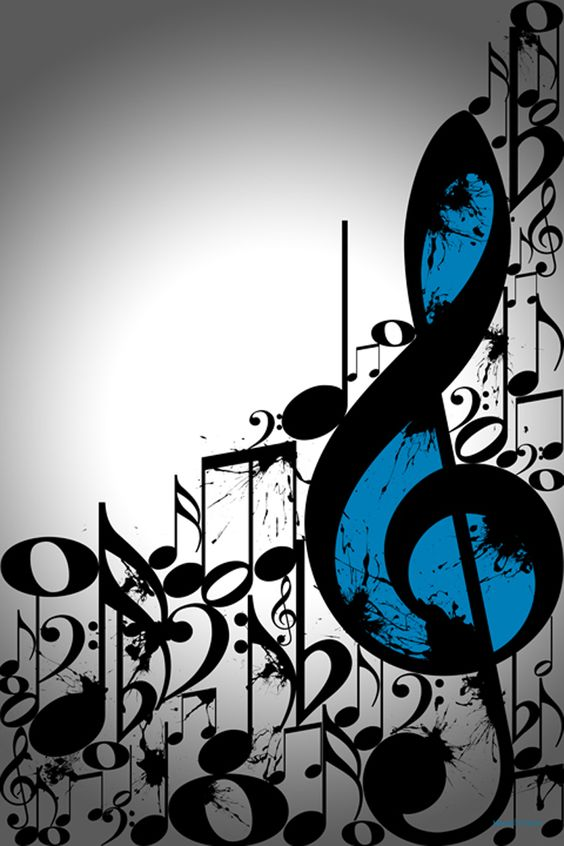
\includegraphics[width = 250px]{./images/deb2.jpg}
\end{center}

\end{figure}






\newpage

\tableofcontents

\newpage

\section{Introduction}

\vspace{1cm}

\subsection{Problématique et but du projet}

\vspace{1cm}

L'idée est de réaliser un petit logiciel pour initier les débutants au solfège. Il fallait donc au départ restreindre le programme,
le domaine de la musique étant assez vaste. Il a donc été décidé collégiallement que le programme aurait un niveau assez faible et 
simple, niveau 6e en musique.


\subsection{Interface générale}

\vspace{1cm}

Il faut donc que l'utilisateur sache lire une partition simple en clef de sol, la partition ne contient que deux gammes.

L'outil choisi pour entrer les notes est un clavier de piano. Le piano étant un instrument universel en musique.

Il a également été décidé de représenter les \verb # 
{ }et les b-mol, ceux-ci étant présent dans de très nombreuses partitions, il est donc
important pour un débutant d'en prendre connaissance.


\subsection{Plan}
\begin{itemize}
\item Explications des choix de l'interface
\item Paper prototype et compte rendu des essais
\item Test du logiciel par des cobayes
\end{itemize}

\newpage
\section{Différents éléments de l'interface}



\subsection{Portée}
\subsection{Menu}

\subsection{Couleur de fond}
Nous avons choisit de mettre le fond en blanc, le blanc rendant la portée plus visible.
Le l'arrière plan du piano est quant à lui légerement grisé pour faire une petite séparation entre la partition et le 
``groupe utilisateur'' (piano + boutons).
\subsection{Piano}
\subsubsection{Pourquoi le Piano ?}
Nous avons choisit de représenter uniquement un piano comme instrument, le métalophone étant très similaire, nous avons
jugé inutile d'en faire un. Pour d'autre instruments tel que le trombonne, les notes auraient été plus difficiles à représenter,
moins parlantes. Le logiciel doit rester simple et pour débutants.
\subsubsection{Interactions}
Quand l'utilisateur appuie sur une touche du piano (avec la souris ou le clavier),
le programme lui confirme son action par une réponse visuelle et auditive.
En effet, la note est jouée et la touche du piano est enfoncée. De plus si l'utilisateur était en plein test sur une partition,
le curseur avance à chaque note tapée.
\subsubsection{Couleurs}
Les couleurs sont bien évidemment noires et blanches comme un piano normal. Nous avons décidé de donner un effet de lumière 
sur la partie haute du piano, les touches noires étant donc blanchies aux sommets. Ceci est un choix purement esthétique et 
apporte un effet plus réaliste au piano.
\subsubsection{Bulle d'information}
Pour chaque touche du piano, si l'utilisateur peut afficher la bulle d'information (tooltip), qui lui indiquera le nom de la 
note et son raccourci clavier. Eh oui, il y a des raccourcis clavier !
\subsection{Raccourcis clavier}
Le but du logiciel est d'apprendre les bases du solfège, mais de les apprendre le plus professionnellement possible.
Il ne sagit donc pas de savoir lire des partitions simple mais de les lire rapidement !
Et pour savoir si l'utilisateur lit une partitions rapidement, il faut qu'il ait pu la jouer rapidement.
Jouer une partition à la souris étant particulièrement sportif et imprécis lorsque l'on joue rapidement, il est nécessaire
de pouvoir la jouer avec le clavier, comme un musicien aurait fait avec un vrai piano.
\subsection{Affichage des raccourcis}
Si chaque touche du piano correspond à une touche du clavier, il serait judicieux d'indiquer à l'utilisateur quelles sont les touches
qui sont associées. Et ceci sans avoir à afficher les bulles d'informations les unes après les autres. Nous avons donc décidé d'implémenter
un moyen d'afficher sur chacune des notes, son raccourci clavier. Cette fonction est lancé par un bouton situé à proximité du piano, ce qui
est évident puisque la fonction agit sur le piano (principe de chépakoi).
Ce bouton est réprésenté par un clavier, ce qui est assez parlant pour un utilisateur qui aurait envie d'utiliser son clavier 
pour jouer du piano.
Bien sûr, au cas où, une bulle d'information indique ce que fait ce bouton si un utilisateur moins futé se posait la question.
\subsection{Affichage du nom des notes}
De façon similaire, nous avons décidé d'implémenter une fonction indiquant la note de chaque touche. Le bouton qui la lance est lui 
aussi proche du piano. Par soucis de symétrie (et donc de confort visuel des utilisateurs), il est situé de l'autre coté de son semblable.
\'A quoi doit ressembler ce bouton: un petit dessin de clé de sol, avec les notes ``do re mi'' écrites est assez communiquant puisque
l'utilisateur peut voir le nom des trois premières notes sur ce bouton. Bien sur si ce n'est pas assez évident, le bulle d'information
est là.
Une question se pose alors : est-il possible d'afficher les raccourcis et les notes en même temps.
Oui, pourquoi pas après tout, si l'utilisateur en a envie, il ne faut pas l'en empêcher. Et ceci est tout à fait justifié si 
l'utilisateur débute avec le logiciel et le piano.
Cependant, nous n'avons pas pu l'implémenter sur notre programme car nous n'avons pas réussi à tout faire tenir sur la largeur de la touche
tout en étant lisible, ni à écrire sur plusieurs lignes dans la touche. Le temps qui nous était imparti étant assez court.
\subsection{Masquer les options}
\subsubsection{Pollution visuelle}
Certains utilisateurs, sûrement une majorité, une fois qu'ils seront familiers avec les notes et les raccourcis, ne voudront plus 
être embêtés par ces deux boutons qui ne leurs sont plus d'aucune utilité, nous avons donc décidé de pouvoir les cacher en décochant
une option.
\subsubsection{Optimisation de l'espace}
Ces deux boutons disparus, il reste de la place innocupée de chaque coté du piano, il est donc judicieux d'augmenter la taille 
du piano en conséquence, ce qui donne un meilleur confort visuel.

\subsubsection{Nom}
Cette fonction permettant d'améliorer l'espace de saisie des notes doit avoir un nom, pour indiquer à l'utilisateur ce qu'il va se 
passer. Le terme ``options d'affichage'' est plutôt parlant et à proximité du piano, il est probable que les options concernent le 
piano.
Le terme ``options'' lui est plus court mais il est moins précis. Quelles sont ces options ? Des touches supplémentaires ?
\subsection{Note de fin de session}
\subsection{Progression}
\subsection{Choix de partitions}
\subsection{Aide pour les débutants}
bouton ``solutions''
\subsection{Tutoriel au premier lancement}
Avec un personnage professeur accompagnant, pas trop humain.

\subsection{Différents logs pour différentes analyses = Compte rendu du jeu}
genre le mec il a mit longtps a trouvé tel note (difftime) ou bien il se trompe souvent pour telle autre note.




\section{Paper Prototype}

\section{Test du logiciel par des cobayes}
\section{Conclusion}
amélioration traduction des notes: donc passage qwerty aussi.
\end{document}

